\subsection{An Active Tracking System using IEEE 802.15.4-based Ultrasonic Sensor Devices}

В документ \cite{yonei} е имплементирана система за следене на обект в пространството използвайки IEEE 802.15.4 базирани ултразвукови сензори.
IEEE 802.15.4 се използва главно в безжичните сензорни мрежи заради ниската консумация на енергия и бързия обмен на информация между компонентите на системата \ref{fig:yoneiFig}. Системата съдържа 1 движещ се компонент. Координатите на движещия се компонент се изчисляват чрез използване на трилатерация.  Описани са 2 категории системи за обработка и изпращане на ултразвукови сигнали \cite{sysTypes}:

\begin{enumerate}
    \item Активни - движещите компоненти излъчват сигнал, а статичните компоненти получават сигнала и го обработват.
    \item Пасивни - движещите компоненти не излъчват сигнал, а получават сигнал, с който се определя разстоянието до различните получатели.
\end{enumerate}

\begin{figure}
    \centering
    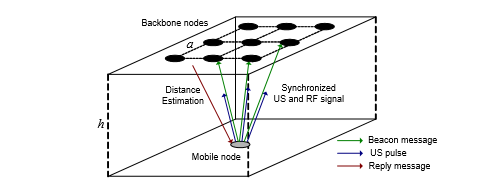
\includegraphics{yonei}
    \caption{Диаграма на разработената система}
    \label{fig:yoneiFig}
\end{figure}


Системата, която е разработена е класифицирана като активна.За коректно пресмятане на координатите на движещия се компонент се изискват измервания от поне 3 бр. статични компонента.

